\documentclass[slidetop]{beamer}
\usetheme{Copenhagen}

\usepackage[utf8x]{inputenc}
\usepackage[francais,french]{babel}
\usepackage{fontenc}
\usepackage{graphicx}
\usepackage{url}
\usepackage{amssymb}
\usepackage{default}

\newcommand{\coq}{Coq~}
\newcommand{\coqtop}{Coqtop~}
\newcommand{\coqide}{CoqIDE~}
\newcommand{\coquille}{\textsc{Coquille}~}
\newcommand{\coqcode}[1]{\texttt{#1}}

\date{Lundi 4 Janvier 2010}
\title{Rapport du projet \coquille}
\author{M1 Informatique Fondamentale - ENS Lyon}

\begin{document}

\begin{frame}[plain]
    \maketitle

    \begin{figure}[ht]
        \begin{minipage}[b]{0.4\linewidth}
            \centering
            
\includegraphics[width=0.4\textwidth]{../images/common/poussin.png}
        \end{minipage}
        \hfill
        \begin{minipage}[b]{0.4\linewidth}   
            \centering
            \includegraphics[scale=0.1]{../images/common/ens.jpg}
        \end{minipage}
    \end{figure}
\end{frame}

\begin{frame}[plain]
    \tableofcontents
\end{frame}

\section{Le projet Coquille en g\'en\'eral}
\documentclass[slidetop]{beamer}

\usepackage[utf8x]{inputenc}
\usepackage[francais,french]{babel}
\usepackage{fontenc}
\usepackage{graphicx}
\usepackage{url}

\usetheme{Copenhagen}
\usepackage{amssymb}

\newcommand{\coquille}{\textsc{Coquille}}
\newcommand{\coqcode}[1]{\texttt{#1}}

\date{10 novembre 2009}
\title{Rapport du projet \coquille{}}
\author{M1 Informatique Fondamentale ENS Lyon}

\usepackage{default}

\begin{document}
\section{Introduction}
\begin{frame}
\maketitle
\center

\includegraphics[width=0.25\textwidth]{poussin.png}

\end{frame}

\begin{frame}
\tableofcontents

\end{frame}

\section{Présentation}
\begin{frame}
Coquille : Coq User-Interactive Library Learning Expert

Objectifs :
\begin{itemize}
  \item Objectif: automatiser la résolution des exercices de mathématiques des classes préparatoires.
    %% à propos, il faut changer les objectifs
  \item Créer les bibliothéques correspondant aux mathématiques de classes préparatoires dans Coq. 
  \item Rendre Coq accessible aux mathématiciens. % non forcément experts en calcul des constructions et en théorie des types. 
\end{itemize}


\end{frame}



\section{WP Preuves et tactiques}
\begin{frame}
\frametitle{WP Preuves et tactiques} 

Le but du WP preuves:
\begin{itemize}
  \item établir une liste de théorèmes vus en classes préparatoires en: 
  \begin{itemize}
    \item algèbre,
    \item analyse,
    \item topologie,
    \item arithmétique.
  \end{itemize}
  \item formaliser les thèorèmes en Coq pour les prouver.
  \item proposer des tactiques évoluées d'aide aux prouveurs. 
  %des tactiques d'aide ?
\end{itemize}

\end{frame}


\begin{frame}
 
Quelques jolis résultats:
\begin{itemize}
  \item R est indénombrable.
  \item L'axiomatique des réels implique le principe de Markov.
  \item La limite de zeta (2) est pi²/6.
  %zeta(2) est une constante !
  \item Convergence de suites réelles et construction de limites.
\end{itemize}
\end{frame}

\begin{frame}
De nouvelles bibliothèques:
\begin{itemize}
  \item Arithmétique.
  \item Topologie (définition de nombreuses typeclass de base, recherche de définitions les plus générales possibles).
    %ça a changé, ce n'est pas que de la topologie
  \item suites et séries réelles et complexes.
  \item Définition du corps des complexes, résultats de base.
    %on ne parle pas de concepts.
  \item Formalisation des séries entières et développements sur les rayons de convergence.
\end{itemize}
\end{frame}


\begin{frame}
\begin{itemize}
\item Toute la documentation générée par coqdoc est disponible sur le site du projet. 
\item Le respect des conventions de nommage permet une utilisation facilitée.
\end{itemize}
\end{frame}


\section{WP IDE}
\begin{frame}
\frametitle{WP IDE} 
L'objectif du WP IDE est de construire une interface de programmation en Coq plus orientée vers l'aide à la programmation que l'actuel CoqIde.
%% L'AIDE À LA PROGRAMMATION ?
% non, pas "plus orientée vers l'aide" non plus. juste plus élaborée avec plus de fonctionalités, et moins de bug (mais pas pour l'instant)
\end{frame}

\begin{frame}
Ce que Coquille fait et que CoqIde ne fait pas au niveau du code :
\begin{itemize}
    \item Les numéros de ligne.
    \item Le code folding (replier des lignes de code en une seule, pour une preuve par exemple).
    \item Des raccourcis plus "classiques", et personnalisables.
    \item Possibilité de faire "Redo" après des "Undo".
\end{itemize}
\end{frame}

\begin{frame}

Au niveau du langage :
\begin{itemize}
    \item La gestion de Ltac Debug, avec une interface de parcours des résultatsScreenshot
    \item Plusieurs instances de Coqtop, une par onglet ouvert
    \item Un affichage des résultats au choix : classique ou LaTeX-likeScreenshot
    \item L'action "Next/Previous" d'envoi d'une commande est considérée comme une action comme les autres, donc "Undo/Redo" agit dessus
\end{itemize}
 
\end{frame}

\begin{frame}

Ce que CoqIde fait au niveau du code :

\begin{itemize}
    \item Lister les tactiques existantes dans un menu.
    \item Lister les actions disponibles par click droit sur une hypothèse ou un but.
\end{itemize}



\end{frame}


\begin{frame}

Au niveau du langage :

\begin{itemize}
    \item Le Proof Wizard.
%    \item La gestion des Write State / Restore State
    \item La gestion de l'aide.
    \item La gestions de la compilation.
\end{itemize}


\end{frame}



\begin{frame}
\includegraphics[width=1\textwidth]{unicode.png}
%ça ne compile pas ! Ajoutez les images, bordel --> ``attention, des images ont été oubliées'' est plus agréable à lire.
%montrer des choses que ne peut pas faire coquille (quoi ?)
\end{frame}

\begin{frame}
\includegraphics[width=1\textwidth]{ltacdebug.png}
%(ltac debug)
\end{frame}

\section{WP Apprentissage}
\begin{frame}
\frametitle{WP Apprentissage} 
WP Apprentissage
L'objectif de ce groupe de travail est à partir de nombreux exercices, de créer des tactiques spécifiques à ce type d'exercice.
\end{frame}
\begin{frame}

% schéma nécessaire
\begin{itemize}
    \item On utilise un arbre de décision. 
    \item A chaque noeud se trouve une question portant sur les arbres syntaxiques des hypothèses et du but. 
\begin{itemize}
    \item Pour la première question, on ne s'autorise à interroger que les racines.
    \item Ensuite, on s'autorise à interroger les fils des arbres déjà interrogés.
\end{itemize}
\end{itemize}

\end{frame}

\begin{frame}

Les questions sont:
\begin{itemize}
    \item Quel est le token à la racine de l'arbre x?
    \item Est-ce que les arbres x et y ont le même token en racine?
\end{itemize}


Pour choisir la question à poser, 
on calcule la question qui nous donne le meilleur rapport "information apportée selon la définition de von Newmann" sur "nombre de réponses". 
On cherche donc à minimiser la taille de l'arbre (et non sa profondeur),
car c'est d'elle que dépend le temps d'exécution et l'occupation de la mémoire.
\end{frame}
\begin{frame}

Résultats
\begin{itemize}
    \item Le parcours d'arbres et le raffinement des données sont utilisables.
    \item L'algorithme d'apprentissage a été réalisé.
\end{itemize}




\end{frame}


\section{WP Communication}


\begin{frame}
\frametitle{WP Communication} 

WP Communication: objectifs
\begin{itemize}
    \item Faciliter la coordination des autres groupes de travail.
    \item Promouvoir le projet et ses résultats auprès de potentiels utilisateurs.
\end{itemize}


\end{frame}


\begin{frame}

Les principales réalisations de ce groupe de travail sont:
\begin{itemize}
 
    \item les rapports. %CHECK ! ah ce n'est pas matthieu qui les a fait ? reponse: chefs de WP rédigent --> WP communication redaction globale --> Matthieu relecture et modification --> Enseignant
    \item cette présentation.
    \item des formations HTML et Latex. %QUOI ????
    \item le site internet.

\end{itemize}
\end{frame}



\begin{frame}
%% intérêt limité de cette liste ?
Un site internet a été réalisé et comporte:
\begin{itemize}
    \item Un forum 
    \item Un wiki
    \item Une présentation du projet 
    \item Nos résultats
    \item Une page de contacts
    \item La documentation de Coquille %NON. N'en déplaise à Eddy, il n'y a pas qu'une documentation de coquille
     % S'il s'agit de l'IDE voici encore une raison pour CHANGER DE NOM POUR L'IDE !!
\end{itemize}


\end{frame}



\section{Bibliographie}
\begin{frame}
\frametitle{Bibliographie} 

 \begin{itemize}
\item [1] http://coq.inria.fr/stdlib/ [la coq standard library]
\item [2] http://c-corn.cs.ru.nl/documentation/toc.html% [les modules disponibles dans Corn]  AH? Parce qu'on a utilisé C-Corn ?
\item [3] http://graal.ens-lyon.fr/coquille/
\item [4] http://perso.ens-lyon.fr/jeanmarie.madiot/coquille/forum % Utile ?
\item [5] http://coquille.wikispot.org/ %% OBSOLÈTE ! Et très utile ...
\item [6] Artifical intelligence, a modern approach, S. Russel P. Norvig

\end{itemize}
\end{frame}


%\section{Conclusion}
%\begin{frame}
 
%\end{frame}

\end{document}


\section{Le WP preuves}
\section{Logique}

\subsection{Indénombrabilité de $\mathbb{R}$ (\coqcode{Runcountable})}

\subsubsection{Motivations}

Le résultat d'indénombrabilité de $\mathbb{R}$ est un résultat fondamental en théorie des ensembles. À ce qu'il semble, il n'a toujours pas été démontré en \Coq{} avec l'axiomatique classique des réels\footnote{Cependant, il en existe une preuve dans C-Corn.}. Quoi qu'il n'ait pas d'intérêt en lui-même au sein d'une bibliothèque d'analyse réelle, ce théorème mérite clairement de figurer parmi les résultats de \coqcode{Rlogic}.

\subsubsection{Énoncé et preuve}

Ce théorème se présente sous deux formes, l'une plus forte que l'autre :
$$\begin{array}{ll}
\mathtt{R\_uncountable\_strong} :& \forall f : \mathbb{N}\rightarrow\mathbb{R}, \forall x < y, \{r\mid\forall n\in\mathbb{N}, r \neq f(n) \wedge\ r\in[x, y]\}\neq\emptyset\\
\mathtt{R\_uncountable} :& \forall f : \mathbb{N}\rightarrow\mathbb{R}, \{r\mid\forall n\in\mathbb{N}, r \neq f(n)\}\neq\emptyset
\end{array}$$

La preuve n'utilise pas la version générale de l'argument diagonal de Cantor, beaucoup trop dur à formaliser en \Coq{}, mais utilise la première preuve de ce résultat que Cantor ait fourni. Elle repose sur un argument purement topologique, à savoir la complétude de $\mathbb{R}$.

\subsection{Implications classiques de l'axiomatique réelle (\coqcode{Rmarkov})}

\subsubsection{Motivations}

L'axiomatique réelle de \Coq{} est \emph{classique}, en ce sens où elle permet de prouver des propriétés que la logique intuitionniste (et par là même \Coq{} dans le contexte vide) ne permet pas. On ignore encore exactement quelles sont les limites de l'expressivité classique conférée par cette axiomatique.

D'un point de vue logique, ceci nous permet de quantifier ce pouvoir expressif, ce qui est toujours intéressant. D'un point de vue pratique, cela nous permet de tirer des ponts entre les différentes représen\-tations des réels, qu'elles soient constructives ou non.

Une preuve certaine que cette question possède un intérêt est apportée par le fait qu'une partie de notre démonstration a été faite avant nous par des chercheurs il y a quelques mois, et sert de base à un développement très intéressant entre C-Corn et \Coq{}.

\subsubsection{Énoncés}

L'axiomatique réelle nous permet de prouver les deux formules suivantes :
$$\begin{array}{llc}
\mathtt{R\_markov} :& \forall P : \mathbb{N}\rightarrow\mathbb{B}, \neg(\forall n\in\mathbb{N}, P(n)) \Rightarrow \exists n\in\mathbb{N}, \neg P(n) & \text{(MP)}\\
\mathtt{R\_sequence\_dec} :& \forall P : \mathbb{N}\rightarrow\mathbb{B}, (\forall n\in\mathbb{N}, P(n)) \vee \neg(\forall n\in\mathbb{N}, P(n)) & \text{(WLPO)}
\end{array}$$

Le premier est le principe de Markov, le second est le principe d'omniscience limité faible. Il est clair que MP n'est que légèrement classique (même si $\not\vdash_{CIC}\text{MP}$, il est constructif au sens algorithmique du terme), alors que WLPO est violemment classique (il permet de résoudre le problème de l'arrêt).

Contrairement à l'article évoqué précédemment, nous avons montré que le principe de Markov était entièrement déductible de l'axiomatique réelle.

Ce résultat permettrait d'écrire une bibliothèque d'analyse réelle auto-contenue, qui ne ferait pas appel à des axiomes classiques. En effet, la plupart des propriétés analytiques sont séquentielles, et MP et WLPO permettent de manipuler les suites classiquement\footnote{Nous n'avons pas encore trouvé de propriété purement analytique sur $\mathbb{R}$ qui ait besoin de plus de MP et WLPO pour être prouvée. Évidemment, si on accepte l'axiome du choix, c'est une autre affaire.}.

Par ailleurs, nous avons tenté de tirer la quintessentielle moëlle classique de l'axiomatique réelle. Hugo Herbelin pensait que l'on pouvait déduire le fait que $\mathbb{R}$ était archimédien des autres axiomes\footnote{L'axiomatique de \Coq{} suppose explicitement que c'est un corps archimédien.}. Il nous a communiqué une preuve intéressante qui montrait que l'on pouvait déduire le tiers exclu faible (WEM) dans \coqcode{Type} à partir de l'axiomatique des réels :

$$\mathtt{Reals}\vdash\forall A : \mathtt{Prop}, \{\neg A\} + \{\neg\neg A\}$$

L'axiome archimédien et MP sont de fait équivalents\footnote{Nous en avons une preuve.}. Nous avons des indices qui nous laissent penser que cet axiome ne peut pas être réduit aux autres. D'abord, parce que MP et WLPO sont complètement orthogonaux en logique intuitionniste. Ensuite parce que WEM a beau impliquer WLPO, WEM n'implique pas non plus MP. Or l'argument utilisé pour prouver WEM à l'aide de l'axiomatique des réels est peu propice à la généralisation pour MP. En effet, de quelque bord qu'on l'attaque, la technique employée ne donne que des résultats par double négation, ce qui est fâcheux pour MP (on veut justement éliminer cette double négation).

Évidemment, nous n'avons pas de modèle pour prouver cela, mais nous conjecturons que l'on ne peut pas se passer de l'axiome archimédien.

\subsubsection{Développements éventuels}

L'idée de bibliothèque réelle auto-contenue pourrait être complètement implémentée, et cela en expurgeant toutes les références au module \coqcode{Classical} de la bibliothèque \coqcode{Reals}. Cependant, la tâche risque de s'avérer longue pour un résultat à l'intérêt douteux.

\section{Analyse}

\subsection{Suites réelles (\coqcode{Rsequence})}

\subsubsection{Motivations}

Les suites sont parmi les outils de base de l'analyse réelle, et le moins qu'on puisse dire, c'est que la bibliothèque standard de \Coq{} n'est ni très étendue dans ce domaine, ni très cohérente\footnote{Comme à peu près tout \coqcode{stdlib}.}. Il y a donc une masse de travail non-négligeable.

Pour ne pas reproduire les défauts de la bibliothèque standard, nous nous sommes entendus pour suivre à la lettre les conventions de nommages recommandées dans la proposition de Hugo Herbelin\cite{naming_conventions}, même si cela s'avère parfois fastidieux. Nous avons également réparti les lemmes en différentes sous-bibliothèques thématiques afin de garantir une consultation aisée et de rendre possible une utilisation modulaire.

\subsubsection{Contenu de la bibliothèque}

Elle définit des propriétés de base, et opère quelques renommages sur les lemmes de \coqcode{stdlib}. Elle se veut très généraliste, sans pour autant assommer l'éventuel utilisateur sous des monceaux de résultats à la \coqcode{techX}.

\paragraph{Convergence} Nous avons renommé la convergence vers un réel afin de respecter un schéma plus naturel. Nous avons aussi défini formellement la divergence vers l'infini (ce qui n'existe pas de base dans la bibliothèque standard). \coqcode{Rsequence} contient une quantité assez impressionnante de lemmules sur la compatibilité des opérations avec la limite. Ces résultats sont d'ailleurs utilisés par une tactique de décision de convergence.

\paragraph{Relations de Landau} Grands classiques des propriétés séquentielles qui souffrent pourtant de cruelles absences de \coqcode{stdlib}. Nous avons donc défini les relations de Landau petit-o, grand-O et équivalence de suite. Nous en avons montré des propriétés importantes : quasi-ordre, équivalence, compatibilités entre elles, etc. Nous avons en outre montré des compatibilités avec les propriétés à la limite et les opérations usuelles.

\paragraph{Suites usuelles} Afin de rester dans un esprit pratique, notre bibliothèque définit des suites appelées à être utilisées un peu partout : suites constantes, polynomiales, exponentielles et factorielles. Certains résultats de comparaison ont été prouvés, et nous avons aussi décrit leur comportement asymptotique.

\paragraph{Autres} \coqcode{Rsequence} contient des propriétés inclassables, néanmoins fort utiles. On peut compter parmi celles-là le fait que la convergence et les relations de Landau soient asymptotiques, c'est-à-dire que tout lemme permettant de prouver une telle propriété peut être généralisé en montrant que les hypothèses ne sont vérifiées qu'à partir d'un certain rang\footnote{Pour plus de clarté, se référer à \coqcode{Rseq\_asymptotic}.}. Nous avons aussi quelques résultats sur les suites partielles.

\subsection{Séries réelles (\coqcode{Rseries})}

\subsubsection{Contenu de la bibliothèque}

Les séries sont un prolongement naturel des suites, et toutes les définitions sont donc calquées sur celles des suites, notemment celles de convergence, divergence, et les relations de Landau.
En particulier, les liens entre convergence, divergence et les relations de Landau ont été fait et beaucoup de résultats concernent les séries à terme positifs puisque beaucoup de problèmes s'y ramènent.

\subsubsection{Série $\zeta(2)$}

La convergence de la série des inverses des carrés des naturels est une propriété connue. La somme de cette série vaut $\frac{\pi^2}6$ et ce résultat fait partie des résultats d'analyse répandus et démontrés de diverses manières.
\[\sum_{n=1}^{\infty}{\frac1{n^2}} = \frac{\pi^2}6\]

Cependant les preuves de ce résultat sont très calculatoires ce qui les rend difficiles à formaliser. La preuve utilisée dans \coqcode{Rzeta2} utilise la définition de $\pi$ dans la bibliothèque standard sous forme d'une série, celle d'$\arctan$, et a motivé la démonstration de nombreux résultats intermédiaires sur les séries, comme la séparation d'une somme infinie selon la parité de ses termes. Elle a nécessité l'introduction des sommes de suites relatives $\mathbb{Z}\rightarrow\mathbb{R}$, ainsi que les sommes doubles correspondantes, parfois privées de leurs termes diagonaux. Une partie non négligeable de la preuve est consacrée à des majorations fines et à du calcul.

\subsection{Séries entières réelles (\coqcode{Rpser})}

\subsubsection{Motivations}

Les séries entières sont une partie intégrante du programme des classes préparatoires. Elles sont pratiquement totalement absentes de la bibliothèque standard (une notation \coqcode{Pser} traduit le fait que la suite des sommes partielles converge mais les rayons de convergence ne sont nullement formalisés). Leur forme très particulière permet de plus de démontrer des théorèmes puissants sans hypothèses trop restrictives.

On pourrait en déduire la dérivabilité et la continuité de certaines fonctions de la bibliothèque standard ($\exp$, $\cos$, $\sin$) qui sont actuellement prouvées « à la main » et qui utilisent des hypothèses inutiles\footnote{Les preuves de dérivabilité de $\cos$ et de $\sin$ dépendent par exemple de l'axiome surnuméraire $\sin\left(\frac{\pi}{2}\right) = 1$.}.

\subsubsection{Définitions}

Une partie importante de nos deux premières semaines de travail a été de trouver les définitions des concepts nous assurant une manipulation aisée de ceux-ci (elles ont fait l'objet de nombreuses retouches au fur et à mesure que nous progressions dans les preuves et que nous constations leurs imperfections).

Nous avons abouti à des représentations très satisfaisantes dont, entre autres, les suivantes :

\paragraph{Série entière} On choisit de représenter la série entière $\sum_{n\in \mathbb{N}} a_n z^n$ par la suite $\left(a_n\right)_{n\in \mathbb{N}}$. Les fonctions \coqcode{gt\_Pser} et \coqcode{gt\_abs\_Pser} sont respectivement de la forme $\lambda a_n.\lambda x.\lambda n.a_n x ^ n$ et $\lambda a_n.\lambda x.\lambda n.\left|a_n x ^ n\right|$ et permettent donc de parler aisément des sommes partielles en n'ayant que la suite $\left(a_n\right)_{n\in \mathbb{N}}$ en paramètre.

\paragraph{Rayon de convergence} Le rayon de convergence $\rho\left(a_n\right)$ est défini de la manière suivante :

$$\rho\left(a_n\right) = \sup \lbrace r \mid (a_n r^n)_{n\in \mathbb{N}} \text{ est bornée} \rbrace$$

\noindent On utilise, en pratique, une version plus faible : \coqcode{Cv\_radius\_weak} $a_n$ $r$ $\stackrel{\Delta}{=}$ $\left(a_n r^n\right)_{n\in \mathbb{N}}$ est bornée.

\subsubsection{Manipulation des définitions}

Quiconque a travaillé sur la bibliothèque des réels peut mesurer à quel point les lemmes très simples permettant de manipuler les définitions sont vitaux. On se donne donc ici quelques lemmes qui permettront de travailler dans des cas particuliers (les démonstrations d'ordre général que nous avons faites par la suite ne nécessitaient pas vraiment la présence de ce genre de choses).

\paragraph{Opérations simples} On prouve que \coqcode{Cv\_radius\_weak} supporte l'affaiblissement\footnote{Si $\left(a_n r^n\right)_{n\in \mathbb{N}}$ est bornée et que $|r'| \le |r|$ alors $\left(a_n (r')^n\right)_{n\in \mathbb{N}}$ l'est également.} et on en déduit que \coqcode{Cv\_radius\_weak} supporte les opérations simples sur les suites (opposé, somme, différence) pour un $r$ bien choisi\footnote{Le $\min$ des $|r|$ des suites en présence fonctionne.}.

\paragraph{Lien entre \coqcode{Pser} et convergence de suite} On prouve qu'il existe un lien entre \coqcode{Pser} (définition pré-existante à notre bibliothèque) et la convergence des sommes partielles.

\subsubsection{Théorèmes fondamentaux}

Nous avons choisi de commencer par implémenter les théorèmes fondamentaux traitant des séries entières : lemme d'Abel, critère de convergence de d'Alembert, caractérisation du rayon de convergence et dérivabilité de la série sur son disque de convergence. C'est là que se situe la majeure partie du travail sur les séries entières (la dérivabilité a notamment fait appel à des lemmes qu'il a fallu démontrer dans \coqcode{RFsequence}).

\paragraph{Lemme d'Abel} Si $\left(a_n r^n\right)_{n\in \mathbb{N}}$ est bornée, alors :
\begin{enumerate}
 \item $$\forall x, |x| < r \Rightarrow \sum_{n\in \mathbb{N}} a_n x^n \text{ admet une limite finie}$$
 \item $$\forall r', 0 \le r' < r \Rightarrow \sum_{n\in \mathbb{N}} a_n x^n \text{ converge normalement sur } D\left(0,r\right)$$
\end{enumerate}

Et une sorte de réciproque : Si $\sum_{n\in \mathbb{N}} a_n x^n$ converge alors \coqcode{Cv\_radius\_weak} $a_n$ $x$.

\paragraph{Critère de d'Alembert} $$\text{Si } \frac{a_{n + 1}}{a_n} \rightarrow \lambda \text{ alors, } \left( \forall r, 0 \le r < \frac{1}{\lambda} \Rightarrow \text{ \coqcode{Cv\_radius\_weak} } a_n~ r\right)$$

\paragraph{Caractérisation du rayon de convergence} On utilise cette fois-ci la définition exacte du rayon de convergence (et non la version affaiblie). Si $\sum_{n\in \mathbb{N}} a_n x^n$ converge simplement et que $\sum_{n\in \mathbb{N}} |a_n x^n|$ diverge, alors $x$ est le rayon de convergence de la série entière.

\paragraph{Dérivabilité de la somme} On démontre que toute série est dérivable (donc continue) sur son disque de convergence. Ce résultat est obtenu est utilisant le fait que la suite des dérivées des sommes partielles converge uniformément (car normalement) sur ce même disque.

Étant donné que la dérivée d'une série entière est une série entière (on a d'ailleurs explicité la fonction \coqcode{An\_deriv} ($\lambda a_n.(n+1)a_{n+1}$) qui donne la suite associée à la série dérivée), on vient de prouver que toute série entière est $C^{\infty}$ sur son disque de convergence.

\subsubsection{Séries de Taylor}

La bibliothèque contient également quelques développements en série de Taylor des fonctions usuelles. Ces résultats se trouvent dans le fichier $\coqcode{RTaylor}$.

\subsection{Intégrales de Riemann réelles (\coqcode{Rintegral})}

\subsubsection{Motivations}
	La librairie standard contient les bases sur le sujet, mais les lemmes et définitions sont peu maniables et la convention de nommage est loin d'être respectée puisqu'il est impossible d'inférer le nom d'un lemme et inversement de savoir ce que fait un lemme dont le nom est du type \coqcode{RiemannInt\_P42}.
	Nous nous sommes donc attachés à fournir des lemmes et des définitions de plus haut niveau à partir des résulats existants tout en essayant de respecter les conventions de nommage.

\subsubsection{Définitions et notations}
	Nous ne manipulons ici que des intégrales réelles définies sur des intervalles. \coqcode{Rint f a b I} signifie que la fonction \coqcode{f} est intégrable entre \coqcode{a} et \coqcode{b} (\emph{i.e.} existence d'une preuve) et que sa valeur est \coqcode{I}. Cette définition est similaire à celle donnée pour la convergence des suites et des séries : la valeur de l'intégrale est un argument et non pas une valeur donnée par une fonction.
	
	\subsubsection{Lien avec les séries}
		Nous avons fait le lien entre intégrales et séries, ce qui a entre autre permis de donner un équivalent de la série harmonique.
	
\subsubsection{Propriétés de base}
	La bibliothèque contient les résultats concernant les propriétés algébriques des intégrales (somme, multiplication par un scalaire) ou les manipulations des bornes (échange des bornes, thèorème de Chasles, intégrale sur un sous-intervalle).
	
	\subsubsection{Autres résultats}
	Quelques propriétés d'inégalité (comme Cauchy-Schwartz ou l'inégalité de la moyenne) sur les intégrales sont maintenant contenues dans la bibliothèque, tout comme d'autres résultats forts comme la nullité d'une fonction continue, positive et d'intégrale nulle ou encore le théorème fondamental de l'analyse. 
	Ce dernier était en effet déjà démontré dans la bibliothèque standard, mais ses hypothèses étaient trop fortes (en particulier, la fonction devait être $\mathcal{C}^1$ sur $\mathbb{R}$, bien que l'on ne l'intègre que sur un intervalle. Ceci a permis de donner la valeur de nombreuses intégrales usuelles comme les polynômes ou les fonctions trigonométriques.
	
\subsection{Complexes (\coqcode{Complex})}


\subsubsection{Motivations}

L'analyse complexe est une importante partie du programme des classes préparatoires. Il est donc absolument nécessaire de définir les complexes proprement et de développer un très grand nombre de lemmes permettant de manipuler les concepts de base. Ce sont ces lemmes qui permettent ensuite de développer des preuves en évitant de revenir trop souvent aux axiomes (ce qui est très lourd).

\subsubsection{Définition et notations}

Les complexes ont été définis comme une paire de réels. Ainsi, aucun axiome n'a été ajouté : on se base uniquement sur l'axiomatique des réels.

Nous avons défini une fonction de ($R \rightarrow R \rightarrow C$) afin de pouvoir créer des complexes. Cette fonction s'est vu associer la notation \coqcode{+i}, ainsi un complexe peut s'écrire sous la forme \coqcode{a +i b}. Nous avons aussi permis l'utilisation des numérables à l'aide d'une coercion de $\mathbb{R}$ dans $\mathbb{C}$.\\
Nous avons tenté d'utiliser des définitions analogues à celles utilisées dans les réels lorsque cela était possible pour faciliter l'utilisation de nos bibliothèques.

\subsubsection{Description}

\begin{description}
 \item [Bases :] Définitions, projecteurs et injections des entiers et des réels.
 \item [Fonctions de base] : Puissance entière, norme et lemmes de manipulation (réécriture, majorations).
 \item [Analyse complexe :] Continuité et dérivabilité.
 \item [Polynômes :] Lemmes sur des polynômes de degré 2 permettant de résoudre certains problèmes dans les réels.
 \item [Trigonométrie :] Existence de la représentation polaire et formule d'Euler.
 \item [Suites Complexes:] Définition et lemmes sur les suites ainsi que les séries et séries entières.
\end{description}

\subsection{Propriétés de $\mathbb{C}$ et fonctions de base}

\subsubsection{Motivations}

Il parait essentiel si l'on veut définir les complexes de façon à ce qu'ils soient utilisables d'écrire des petits lemmes sur la compatibilité de l'addition, multiplication, division etc. Dans la même optique d'utilisabilité de la bibliothèque complexe, nous avons créé des tactiques permettant d'utiliser les choses connues dans les réels.

\subsubsection{Description}

Dans \coqcode{Cbase}, on démontre que les opérations d'addition et de multiplication que l'on a définies font de $\mathbb{C}$ un corps. Cela nous donne un début de bibliothèque de lemmes utilisables pour prouver des théorèmes dans $\mathbb{C}$.

Nous avons des tactiques permettant de passer dans les réels : 
\begin{itemize}
 \item \coqcode{CusingR} détruit tous les nombres complexes de l'environnement et fait \coqcode{auto} sur les réels ainsi créés ;
 \item \coqcode{CusingR\_f} fait la même chose que \coqcode{CusingR} mais fait \coqcode{field} au lieu de \coqcode{auto} ;
 \item \coqcode{CusingR\_simpl} est utilisable sur une égalité. On passe dans les réels à travers \coqcode{Cre} et \coqcode{Cim} respectivement fonctions d'obtention de la partie réelle et complexe.
\end{itemize}

\subsection{Propriétés de $\mathbb{C}$ (\coqcode{Cmet}, \coqcode{Ctacfield})}

\subsubsection{Motivations}

La bibliothèque standard propose des résultats généraux sur certaines structures. Afin d'utiliser au mieux ces résultats, on doit évidemment prouver que $\mathbb{C}$ remplit les conditions nécessaires.

\subsubsection{Description}

\begin{itemize}
 \item \coqcode{Cmet} On démontre que $\mathbb{C}$ est un espace métrique.
 \item \coqcode{Ctacfield} On démontre que $\mathbb{C}$ est un anneau, puis un corps. Cela nous permet d'obtenir les tactiques \coqcode{ring\_simplify}, \coqcode{ring}, \coqcode{field\_simplify} et \coqcode{field} qui sont très utiles pour résoudre des égalités (ces tactiques sont compatibles avec \coqcode{Cpow} qui est la puissance entière).
\end{itemize}


\subsection{Des fonctions et définitions de base}

\subsubsection{Motivations}

Pour montrer des théorèmes intéressants, nous avons eu besoin de créer quelques fonctions de base et beaucoup de lemmes pour pouvoir utiliser ces fonctions. %TODO Très bof, ça. Ben modifiez le Bordel !

\subsubsection{Description}

\begin{itemize}
 \item \coqcode{Cpow} est l'équivalent de \coqcode{pow} pour les nombres complexes.
 \item \coqcode{Cnorm} est la fonction renvoyant la norme d'un nombre complexe (on a notamment prouvé l'inégalité triangulaire).
 \item \coqcode{sum\_f\_C0} est la somme finie.
\end{itemize}


\subsection{Suites complexes (\coqcode{Csequence})}

\subsubsection{Motivations}

Il est nécessaire de disposer de résultats de base sur les suites à valeurs complexes pour pouvoir construire une bibliothèque traitant des séries entières dans $\mathbb{C}$.

\subsubsection{Description}

Cette bibliothèque est la petite s\oe{}ur de la bibliothèque sur les suites à valeurs réelles. Elle ne fait que transposer les théorèmes concernant la convergence des suites et la compatibilité de ces convergences avec les opérateurs de base (opposé, inverse, somme, différence, multiplication).

\subsection{Séries entières complexes (\coqcode{Cpser})}

\subsubsection{Motivations}

Les séries entières sont la base de la trigonométrie telle qu'elle est faite en \Coq{}. Le programme de classes préparatoires se base aussi largement sur ce genre de série. Il apparait donc essentiel de définir les séries entières en \Coq{}.

\subsubsection{Description}



\subsubsection{Application}

On pourrait se baser sur cette bibliothèque pour définir les fonctions trigonométriques complexes ou encore l'exponentielle complexe.

\subsection{Résultats intéressants}

\subsubsection{D\'eveloppement en sommes finies de $(a + b) ^ n$}

Ce résultat semble déjà avoir été démontré dans les réels sous le nom de \coqcode{binomial}. Il n'est pas possible de le réutiliser directement pour prouver le résultat dans les complexes à cause de la notation \coqcode{+i} qui fait apparaître de nouvelles difficultés.

\subsubsection{Existence de racines d'un trinôme}

Dans \coqcode{Croot\_n}, nous nous sommes intéressés aux polynômes. Nous avons entre autres prouvé l'existence d'une racine carrée pour tout nombre complexe. On a aussi montré que tout polynôme complexe admet 2 racines.

On a déduit l'existence ou non de racines pour un polynôme de degré 2 dans les réels ainsi que la positivité lorque $\Delta < 0$.

\subsubsection{Représentation polaire}

Nous avons défini les complexes comme des paires de réels. Nous ne savions pas \emph{a priori} qu'il existait une représentation polaire pour ces complexes. Nous l'avons donc montré. Ce résultat fait intervenir l'arctangente (cf. \coqcode{Reals}).

\subsubsection{Formule d'Euler}

Nous avons défini l'exponentielle complexe comme une somme infinie (la même définition que l'exponentielle réelle). Nous avons donc montré la formule d'Euler : $ e^{ i\theta } = \cos \theta + i\sin \theta $

\subsubsection{Produit de Cauchy complexe}%TODO à commenter ou pas (theoremme de Mertens)

\subsubsection{Existence de la racine n-ième d'un nombre complexe}
%TODO à reformuler
Nos résultats précédents nous ont permis de montrer :
Pour tout nombre complexe $z$ et tout entier $n$ supérieur à $0$, il existe un nombre complexe $z1$ tel que $z1 ^ n = z$.

\section{Topologie}

\subsection{Objets topologiques (\coqcode{Topology})}

\subsubsection{Motivations}

L'approche standard de définition des objets mathématiques dans \Coq{} est basée sur la définition constructive d'éléments moins généraux vers d'autres plus généraux. Les principes constructifs justifient cette approche. Cependant certains objets ne peuvent être construits, par exemple dans \coqcode{Reals}, le fait que $\mathbb{R}$ est un corps n'est pas une propriété mais un axiome.

Ainsi pour faciliter la définition d'objets plus généraux, on peut tenter de définir les objets les plus généraux dans un premier temps. Un besoin suggéré par la manipulation des suites, séries ou même des complexes est une homogénéisation des tactiques pour simplifier les expressions qui supportent des propriétés de groupe, d'anneau ou encore d'espace vectoriel. On cherche à généraliser la notion d'espace.

\subsubsection{Description}

Dans \coqcode{Topology} sont définis les espaces topologiques. Il est nécessaire d'introduire la notion d'union d'une famille d'ensembles indexée par un ensemble quelconque (dénombrable ou non). On y montre que les topologies discrète $(V,\mathcal{P}(V))$ et triviale $(V,\{\emptyset,V\})$ sont effectivement des topologies, et on définit la notion de séparation (T2, de Hausdorff).

Dans \coqcode{Metrics} on définit les espaces métriques. Notamment, il y est prouvé qu'un espace métrique définit une topologie (dont les ouverts sont les unions de boules ouvertes) et que l'espace topologique ainsi construit est séparé.

La notion de continuité est introduite dans \coqcode{Continuity}, dans la version topologique et la version métrique. On y montre que sur un espace métrique la topologie induite par la distance définit la même continuité que la continuité métrique.

Les espaces vectoriels sont introduits dans \coqcode{Vectors}, ainsi que la notion de base d'un espace. La définition du produit scalaire est dans \coqcode{Inner\_product}.

Une importante attention est portée à la réutilisation des objets car il s'agit typiquement d'objets sujets à l'héritage. Par exemple, un espace hermitien est un espace vectoriel sur $\mathbb{C}$, de dimension finie et muni d'un produit scalaire. L'utilisation des \emph{typeclasses} semble incontournable.

%TODO : notes sur la lourdeurs des notations et des définitions, notamment sur la notion de fonction
%TODO : notes sur la nécessité d'une bibliothèque qui définit mieux les ensembles, (pourquoi pas un peu de théorie des ensembles, mais on sort du cadre initial du projet

\subsubsection{Développements futurs}

Comme \coqcode{Vectors} pourra donner naissance à des tactiques de manipulation spécifiques aux espaces vectoriels, %% Devrait être fait dans hierarchy
l'héritage (l'ajout d'un produit scalaire par exemple) pourra augmenter le nombre de tactiques et de théorèmes disponibles. Le but inhérent est d'écrire et de prouver des théorèmes utilisant des objets les plus généraux possibles pour étendre leur champ d'application.

Prévisions (l'ordre est indicatif de la priorité) :
\begin{itemize}
  \item suites de Cauchy (cas métrique) ;
  \item complétion ;
  \item compacité ;
  \item dimension finie, application ; %DUR
  \item cas de $\mathbb{R}$ ;
  \item $\sigma$-algèbres, mesure ;
%  \item différentiabilité ; % -> Hierarchy, éventuellement
  \item espace vectoriel topologique ; %sort du cadre
  \item axiome du choix, équivalents, conséquences ; %sort du cadre
\end{itemize}

\section{Arithmétique}

\subsection{Motivations}

L'arithmétique est une branche difficile des mathématiques dont la plupart des preuves reposent soit sur des résultats difficile d'algèbre soit sur des preuves élémentaires mais dont de nombreux éléments de la preuves sont « laissés au lecteurs » ou peu formels. De plus, de nombreux éléments considérés comme élémentaires en théorie des nombres (coefficients binomiaux, manipulations de sommes finies, résultats sur la primalité, etc.) demandent un grand efforts pour être formalisés et pour être utilisés.

Le but de ce dévelopement est de formaliser quelques uns de ces concepts et de les utiliser afin de prouver un résultat non trivial de théorie des nombres, à savoir le petit théorème de Fermat.

\subsection{Description}

Tous les théorèmes traitent des entiers naturels (\coqcode{nat}). Bien que la plupart puisse être étendus au cas des entiers relatifs (\coqcode{Z}), ceux-ci ne sont pas nécessaires pour obtenir ces théorèmes. De plus, la plupart des preuves sont basées sur un raisonnement par induction qui est naturel dans \coqcode{nat} et qui l'est moins dans \coqcode{Z}.

Les dévelopements sur l'arithmétique ont été pensés de façon modulaires, ceux-ci regroupent les thématiques suivantes:
\begin{itemize}
 \item Inductions : généralisation de la récurrence sur \coqcode{nat} à la récurrence à $n$-pas et la récurrence forte.
 \item Fonction puissance : définitions de la mise d'un entier à la puissance d'un autre
 \item Divisibilité : définition de la divisibilité, de la primalité, du plus grand diviseur commun, du plus petit (resp. grand) diviseur premier d'un nombre, décidabilité de la divisibilité\ldots
 \item Sommes et produits finis : définitions et propriétés, notamment sur le fait de « couper une somme en deux »
 \item Coefficients binomiaux : définitions à partir de la relation de Pascal, liens avec l'expression sous forme de factorielles, divisibilité\ldots
 \item Formule du binôme de Newton : preuve du théorème de newton dans le cas où toutes les variables sont des entiers naturels
 \item Petit théorème de Fermat : preuve élémentaire du théorème basé sur la formule du binôme de Newton
\end{itemize}

\subsection{Développements futurs}

Il faudrait étendre ces résultats au cas des entiers relatifs. Une autre direction serait de faire une preuve en utilisant des résultats sur les groupes ou encore de généraliser le binôme de Newton à un anneau commutatif (ce serait alors un résultat d'algèbre).


\section{Le WP IDE}
\begin{frame}
\frametitle{WP IDE} 
L'objectif du WP IDE est de construire une interface de programmation en Coq plus orientée vers l'aide à la programmation que l'actuel CoqIde.
%% L'AIDE À LA PROGRAMMATION ?
% non, pas "plus orientée vers l'aide" non plus. juste plus élaborée avec plus de fonctionalités, et moins de bug (mais pas pour l'instant)
\end{frame}

\begin{frame}
Ce que Coquille fait et que CoqIde ne fait pas au niveau du code :
\begin{itemize}
    \item Les numéros de ligne.
    \item Le code folding (replier des lignes de code en une seule, pour une preuve par exemple).
    \item Des raccourcis plus "classiques", et personnalisables.
    \item Possibilité de faire "Redo" après des "Undo".
\end{itemize}
\end{frame}

\begin{frame}

Au niveau du langage :
\begin{itemize}
    \item La gestion de Ltac Debug, avec une interface de parcours des résultatsScreenshot
    \item Plusieurs instances de Coqtop, une par onglet ouvert
    \item Un affichage des résultats au choix : classique ou LaTeX-likeScreenshot
    \item L'action "Next/Previous" d'envoi d'une commande est considérée comme une action comme les autres, donc "Undo/Redo" agit dessus
\end{itemize}
 
\end{frame}

\begin{frame}

Ce que CoqIde fait au niveau du code :

\begin{itemize}
    \item Lister les tactiques existantes dans un menu.
    \item Lister les actions disponibles par click droit sur une hypothèse ou un but.
\end{itemize}



\end{frame}


\begin{frame}

Au niveau du langage :

\begin{itemize}
    \item Le Proof Wizard.
%    \item La gestion des Write State / Restore State
    \item La gestion de l'aide.
    \item La gestions de la compilation.
\end{itemize}


\end{frame}



\begin{frame}
\includegraphics[width=1\textwidth]{../images/ide/unicode.png}
%ça ne compile pas ! Ajoutez les images, bordel --> ``attention, des images ont été oubliées'' est plus agréable à lire.
%montrer des choses que ne peut pas faire coquille (quoi ?)
\end{frame}

\begin{frame}
\includegraphics[width=1\textwidth]{../images/ide/ltacdebug.png}
%(ltac debug)
\end{frame}


\section{Le WP Apprentissage}
\begin{frame}
\frametitle{Objectifs} 

L'objectif de ce groupe de travail est à partir de nombreux exercices, de créer des tactiques spécifiques à ce type d'exercice.

\end{frame}

\begin{frame}
\frametitle{Arbre de décision}
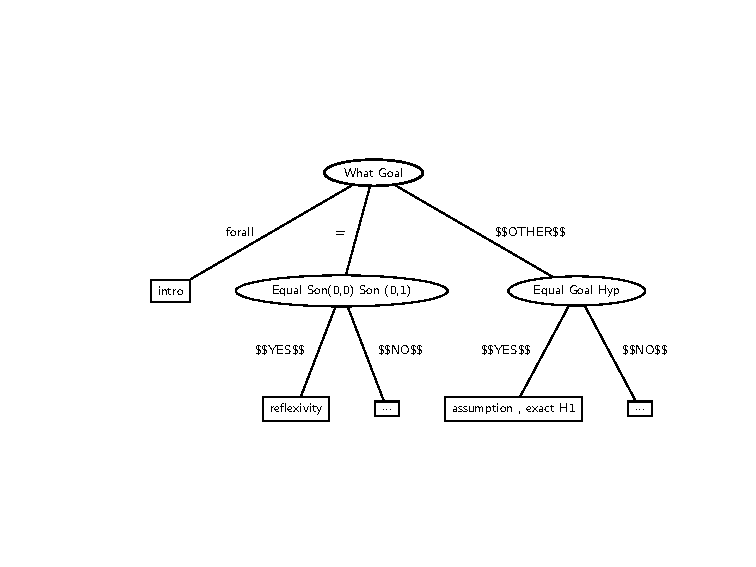
\includegraphics{../images/apprentissage/decision_tree.jpg}
\end{frame}

\begin{frame}
\frametitle{Découpage du workpackage}
\includegraphics[scale=0.2]{../images/apprentissage/organisation_apprentissage.pdf}
\end{frame}


\begin{frame}
  \frametitle{Acquisition}
  «en fonction du contexte (hypothèses+but), quelle tactique ?»
  \begin{itemize}
    \item analyse des fichiers {\tt .v}
      \begin{itemize}
        \item outils existants (XML) : inadaptés (contextes intermédiaires)
        \item lex+yacc : schéma général
        \item \textit{ad-hoc} : identificateurs dans chaque terme
      \end{itemize}
    \item analyse des fichiers {\tt .out} (sortie de coqtop) 
      \begin{itemize}
        \item \textit{ad-hoc} : schéma général très spécifique à coqtop
        \item lex+yacc : termes d'hypothèses et de but
      \end{itemize}
    \item combinaison contextes/tactiques
    \item traitement
      \begin{itemize}
        \item indices des variables dans le contexte (De Bruijn)
        \item forme spécifique à l'algorithme d'apprentissage
      \end{itemize}
  \end{itemize}
\end{frame}



\begin{frame}
\frametitle{L'apprentissage}
  \begin{definition}[entropie]
    L'entropie d'un tirage aléatoire est la longueur moyenne du code pour désigner la réponse : $\sum_{i \in I}{-p_i*\log{p_i}}$
  \end{definition}

  On cherche donc à diminuer l'entropie jusqu'à 0 grâce à des questions. 
 
  De plus, on veut avoir l'arbre le plus petit possible

  On choisit la question qui maximise la diminution d'entropie sur le nombre de réponse.

\end{frame}

\begin{frame}
  \frametitle{Difficultés}
  \begin{itemize}
  \item Grand nombre de questions possibles
  \item Multiplicité des réponses à une même question pour un même exemple
  \item Renumérotation des hypothèses
  \item Questions non fixes
  \end{itemize}
\end{frame}


\begin{frame}
  \frametitle{Pipeau?}
  \begin{itemize}
  \item Supposition d'une distribution représentative \\
    $\rightarrow$ Problèmes très classiques, redondant
  \item Pas l'arbre le plus petit en théorie \\
    $\rightarrow$ En pratique, ça marche
  \item Choix restreint sur les questions\\
    $\rightarrow$ Souvent comme ça qu'on réflechit
  \end{itemize}
\end{frame}


\begin{frame}
  \frametitle{Résultats}
  \begin{itemize}
  \item L'extraction de donnée est faite
  \item L'algorithme d'apprentissage est fait
  \item La décision à partir d'un problème et d'un arbre est faite
  \item Bonus 1 : Traduction en tactique
  \item Bonus 2 : On comprend ``apply H''
  \item Efficace?
\end{itemize}
\end{frame}

\begin{frame}
  \frametitle{Perspectives}
  
  \begin{itemize}
  \item Compréhension des termes : cut ( z + t = 10)
  \item Connexion avec l'IDE
  \item Bases d'exemples sur le net
  \item Update à la volée
  \item Pruning : quand les questions n'ont aucun sens
  \end{itemize}
\end{frame}


\section{Le WP communication}
\begin{frame}
\frametitle{WP Communication} 

WP Communication: objectifs
\begin{itemize}
    \item Faciliter la coordination des autres groupes de travail.
    \item Promouvoir le projet et ses résultats auprès de potentiels utilisateurs.
\end{itemize}


\end{frame}


\begin{frame}

Les principales réalisations de ce groupe de travail sont:
\begin{itemize}
 
    \item les rapports. %CHECK ! ah ce n'est pas matthieu qui les a fait ? reponse: chefs de WP rédigent --> WP communication redaction globale --> Matthieu relecture et modification --> Enseignant
    \item cette présentation.
    \item des formations HTML et Latex. %QUOI ????
    \item le site internet.

\end{itemize}
\end{frame}



\begin{frame}
%% intérêt limité de cette liste ?
Un site internet a été réalisé et comporte:
\begin{itemize}
    \item Un forum 
    \item Un wiki
    \item Une présentation du projet 
    \item Nos résultats
    \item Une page de contacts
    \item La documentation de Coquille %NON. N'en déplaise à Eddy, il n'y a pas qu'une documentation de coquille
     % S'il s'agit de l'IDE voici encore une raison pour CHANGER DE NOM POUR L'IDE !!
\end{itemize}


\end{frame}


\section{Bibliographie}

\begin{frame}{Bibliographie} 
 \begin{itemize}
\item [1] http://coq.inria.fr/stdlib/ [la coq standard library]
\item [2] http://c-corn.cs.ru.nl/documentation/toc.html% [les modules disponibles dans Corn]  AH? Parce qu'on a utilisé C-Corn ?
\item [3] http://graal.ens-lyon.fr/coquille/
\item [4] http://perso.ens-lyon.fr/jeanmarie.madiot/coquille/forum % Utile ?
\item [5] http://coquille.wikispot.org/ %% OBSOLÈTE ! Et très utile ...
\item [6] Artifical intelligence, a modern approach, S. Russel P. Norvig
\end{itemize}
\end{frame}

\end{document}
